% figure1_propC.tex — Proposal C: three-panel matryoshka (zoom-in chain).
%
% (a) Agentic workflow strip — concrete events on a horizontal time axis,
%     with a thin GPU-active KV size bar below. ~1.5 cm tall.
% (b) Tiered offload-repair loop — Active KV (top) / Host buffer (bottom),
%     with evict (dashed, down) and RepairKV (teal, up) arrows; signal s
%     enters RepairKV from above. ~2.5 cm tall.
% (c) RepairKV mechanism (chip-level) — Host before / RepairKV pill /
%     Active after. Ghost slots in host_before show where the K rows
%     came from. ~3.0 cm tall.
%
% Generic — uses "signal s", no Q_2. "Compress P" decoration removed.
% All panels share the same horizontal extent; panel labels at one x.
% Shared preamble for standalone Figure 1 variants.
\documentclass[border=8pt,tikz]{standalone}
\usepackage{amsmath}
\usepackage{amssymb}
\usepackage{tikz}
\usetikzlibrary{arrows.meta,positioning,calc,fit,shapes.geometric,backgrounds}
\usepackage{xcolor}
\usepackage[T1]{fontenc}
\usepackage{mathptmx}
\newcommand{\repairkv}{\textsc{RepairKV}}
\newcommand{\bbase}{\ensuremath{B_{\mathrm{base}}}}
\newcommand{\bmatch}{\ensuremath{B_{\mathrm{match}}}}

\begin{document}
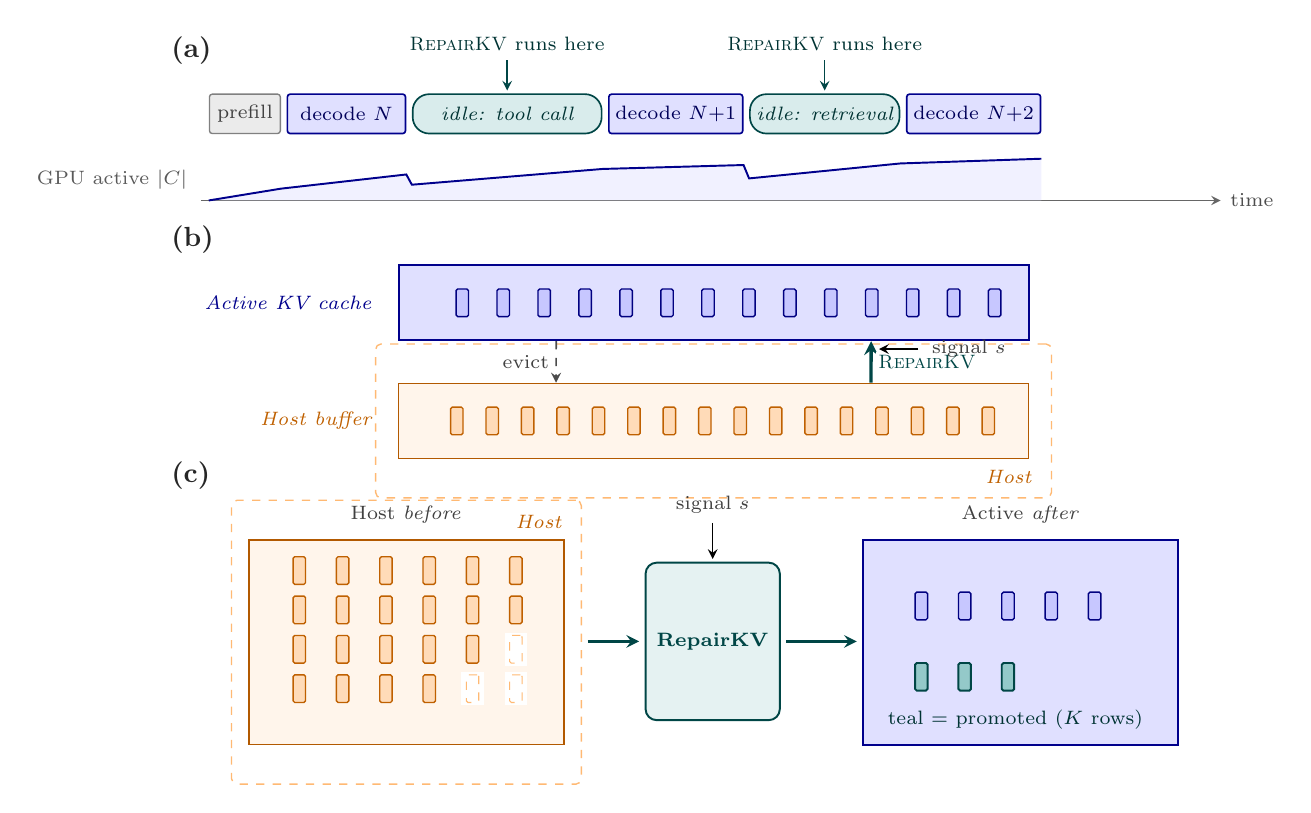
\begin{tikzpicture}[
  >=latex, line width=0.4pt, font=\small,
  % --- shared box styles ---
  box/.style={draw=black, fill=white, line width=0.5pt,
              inner sep=4pt, align=center, minimum height=0.7cm},
  active/.style={box, fill=blue!12, draw=blue!55!black, line width=0.7pt},
  store/.style={box, fill=orange!8, draw=orange!70!black, line width=0.6pt},
  arr/.style={->, line width=0.55pt, draw=black, >=stealth},
  promarr/.style={->, line width=0.95pt, draw=teal!55!black, >=stealth},
  evictarr/.style={->, line width=0.6pt, draw=black!70, dashed, >=stealth},
  arrlabel/.style={font=\scriptsize, text=black!75, fill=white, inner sep=1pt},
  groupbox/.style={draw=orange!55, dashed, line width=0.5pt, rounded corners=2pt},
  grouplabel/.style={font=\scriptsize\itshape, text=orange!75!black},
  panellabel/.style={font=\bfseries, text=black!85},
  rowlabel/.style={font=\itshape\scriptsize},
  % --- chip styles ---
  chip/.style={rounded corners=0.6pt, minimum width=4.5pt, minimum height=10pt,
               inner sep=0pt, line width=0.5pt},
  ghostchip/.style={chip, draw=orange!55, fill=white, dashed, line width=0.4pt},
  gpuchip/.style={chip, draw=blue!50!black, fill=blue!22},
  hostchip/.style={chip, draw=orange!75!black, fill=orange!28},
  promchip/.style={chip, draw=teal!55!black, fill=teal!42, line width=0.7pt},
  rkvpill/.style={draw=teal!55!black, fill=teal!10, line width=0.7pt,
                  rounded corners=4pt, inner sep=4pt, align=center,
                  font=\scriptsize\bfseries, text=teal!55!black},
  % --- timeline events ---
  evprefill/.style={draw=black!50, fill=black!8, line width=0.5pt,
                    rounded corners=1pt, minimum height=0.50cm,
                    inner sep=2pt, align=center, font=\scriptsize, text=black!75},
  evdecode/.style={draw=blue!55!black, fill=blue!12, line width=0.6pt,
                   rounded corners=1pt, minimum height=0.50cm,
                   inner sep=2pt, align=center, font=\scriptsize, text=blue!35!black},
  evidle/.style={draw=teal!55!black, fill=teal!15, line width=0.6pt,
                 rounded corners=6pt, minimum height=0.50cm,
                 inner sep=2pt, align=center,
                 font=\scriptsize\itshape, text=teal!40!black},
  callout/.style={font=\scriptsize, text=teal!40!black, align=center}
]

% =====================================================================
% LAYOUT — y-coords (top to bottom):
%   (a) timeline strip  : y in [4.6, 6.6]
%   (b) tiered loop     : y in [1.6, 4.0]
%   (c) chip mechanism  : y in [-3.2, 1.0]
% Shared horizontal extent: x in [0, 13].  Panel labels at x = -0.5.
% =====================================================================
\def\xLab{-0.5}

% =====================================================================
% Panel (a) — Agentic workflow strip
% =====================================================================
\node[panellabel, anchor=south west] at (\xLab, 6.45) {(a)};

% RepairKV callouts (placed first so they sit above the events)
% Event boxes laid out left-to-right starting at x=0.10 on row y=5.95.
\def\evY{5.95}

\node[evprefill, minimum width=0.9cm, anchor=west] (evP)  at (0.10,\evY) {prefill};
\node[evdecode,  minimum width=1.5cm, anchor=west, right=2pt of evP]  (evD1) {decode~$N$};
\node[evidle,    minimum width=2.4cm, anchor=west, right=2pt of evD1] (evI1) {idle: tool call};
\node[evdecode,  minimum width=1.7cm, anchor=west, right=2pt of evI1] (evD2) {decode~$N{+}1$};
\node[evidle,    minimum width=1.9cm, anchor=west, right=2pt of evD2] (evI2) {idle: retrieval};
\node[evdecode,  minimum width=1.7cm, anchor=west, right=2pt of evI2] (evD3) {decode~$N{+}2$};

% Two RepairKV callouts above idle events
\draw[->, line width=0.55pt, teal!55!black, >=stealth]
     ([yshift=12pt]evI1.north) -- ([yshift=1pt]evI1.north);
\node[callout, anchor=south] at ([yshift=12pt]evI1.north)
     {\repairkv{} runs here};
\draw[->, line width=0.55pt, teal!55!black, >=stealth]
     ([yshift=12pt]evI2.north) -- ([yshift=1pt]evI2.north);
\node[callout, anchor=south] at ([yshift=12pt]evI2.north)
     {\repairkv{} runs here};

% --- Below events: GPU-active KV size bar (polyline + light fill)
\def\baseY{4.85}
\def\maxY{5.40}
\def\xRtl{12.4}  % right end of timeline content (just past evD3)

% baseline + axis
\draw[->, line width=0.5pt, black!60, >=stealth]
     (0.0,\baseY) -- (\xRtl+0.55,\baseY)
     node[right, font=\scriptsize, text=black!70] {time};
\node[font=\scriptsize, text=black!65, anchor=east]
     at (-0.05, 5.12) {GPU active $|C|$};

% Sample x-points at event boundaries
\path (evP.west)  ++(0,0) coordinate (paP);
\path (evP.east)  ++(0,0) coordinate (paPe);
\path (evD1.east) ++(0,0) coordinate (paD1e);
\path (evI1.west) ++(0,0) coordinate (paI1w);
\path (evI1.east) ++(0,0) coordinate (paI1e);
\path (evD2.east) ++(0,0) coordinate (paD2e);
\path (evI2.west) ++(0,0) coordinate (paI2w);
\path (evI2.east) ++(0,0) coordinate (paI2e);
\path (evD3.east) ++(0,0) coordinate (paD3e);

% Heights (in y-units): rise during prefill+decode, dip at evict (idle start),
% snap up after RepairKV.
\fill[blue!10, opacity=0.55]
     (paP   |- 0,\baseY) --
     (paPe  |- 0,5.00) --
     (paD1e |- 0,5.18) --
     (paI1w |- 0,5.05) --     % dip at evict
     (paI1e |- 0,5.25) --     % RepairKV jump
     (paD2e |- 0,5.30) --
     (paI2w |- 0,5.13) --     % dip
     (paI2e |- 0,5.32) --     % RepairKV jump
     (paD3e |- 0,5.38) --
     (paD3e |- 0,\baseY) -- cycle;

\draw[blue!55!black, line width=0.7pt]
     (paP   |- 0,\baseY) --
     (paPe  |- 0,5.00) --
     (paD1e |- 0,5.18) --
     (paI1w |- 0,5.05) --
     (paI1e |- 0,5.25) --
     (paD2e |- 0,5.30) --
     (paI2w |- 0,5.13) --
     (paI2e |- 0,5.32) --
     (paD3e |- 0,5.38);

% =====================================================================
% Panel (b) — Tiered offload-repair loop
% =====================================================================
\node[panellabel, anchor=south west] at (\xLab, 4.05) {(b)};

% Active KV (top, pale-blue rectangle with chips)
\node[active, minimum width=8.0cm, minimum height=0.95cm, anchor=west]
     (bAct) at (2.5, 3.55) {};
% chips inside Active — 14 blue tokens distributed across 8.0cm bar
\foreach \i in {1,...,14}{
  \pgfmathsetmacro{\xc}{2.5 + 0.30 + 0.52*\i}
  \node[gpuchip] at (\xc, 3.55) {};
}

% Host buffer (bottom) inside dashed orange Host group
\node[store, minimum width=8.0cm, minimum height=0.95cm, anchor=west]
     (bHost) at (2.5, 2.05) {};
% chips inside Host — 16 orange tokens distributed across 8.0cm bar
\foreach \i in {1,...,16}{
  \pgfmathsetmacro{\xc}{2.5 + 0.30 + 0.45*\i}
  \node[hostchip] at (\xc, 2.05) {};
}

% Dashed orange Host group around host buffer
\node[groupbox, fit=(bHost), inner xsep=8pt, inner ysep=14pt] (bHostGrp) {};
% Host label INSIDE the dashed group, bottom-right corner
\node[grouplabel, anchor=south east]
     at ([xshift=-4pt, yshift=2pt]bHostGrp.south east) {Host};

% Row labels (left side, outside)
\node[rowlabel, text=blue!55!black, anchor=east]
     at ([xshift=-6pt]bAct.west) {Active KV cache};
\node[rowlabel, text=orange!75!black, anchor=east]
     at ([xshift=-6pt]bHost.west) {Host buffer};

% DOWN arrow: evict (dashed). Place at left third of the bars.
\draw[evictarr]
     ([xshift=-2.0cm]bAct.south) -- ([xshift=-2.0cm]bHost.north);
\node[arrlabel, anchor=east]
     at ([xshift=-2.05cm]bAct.south |- 0,2.80) {evict};

% UP arrow: RepairKV (teal, bold). Right third.
\draw[promarr, line width=1.2pt]
     ([xshift=2.0cm]bHost.north) -- ([xshift=2.0cm]bAct.south);
\node[arrlabel, text=teal!55!black, anchor=west]
     at ([xshift=2.05cm]bAct.south |- 0,2.80) {\repairkv{}};

% Signal s — feeds the RepairKV up-arrow shaft from the right
\node[font=\scriptsize, text=black!75, anchor=west]
     at ([xshift=2.65cm, yshift=-0.10cm]bAct.south) {signal $s$};
\draw[arr, line width=0.55pt]
     ([xshift=2.60cm, yshift=-0.10cm]bAct.south)
     -- ([xshift=2.10cm, yshift=-0.10cm]bAct.south);

% =====================================================================
% Panel (c) — RepairKV mechanism (chip-level)
%   Host before  /  RepairKV pill  /  Active after
% =====================================================================
\node[panellabel, anchor=south west] at (\xLab, 1.05) {(c)};

% Three column geometry:
%   Host before:    x in [0.6, 4.6]   (4.0 cm wide)
%   RepairKV pill:  x ~ 6.5           (1.5 cm wide)
%   Active after:   x in [8.4, 12.4]  (4.0 cm wide)
% Top y = 0.55, bottom y = -2.65 (so dashed group fits with margin).

% Host before (orange container, 4 rows x 6 cols = 24 chips)
\node[store, minimum width=4.0cm, minimum height=2.6cm,
      anchor=north west] (cHostB) at (0.6, 0.55) {};
\node[font=\scriptsize, text=black!75, anchor=south]
     at ([yshift=2pt]cHostB.north) {Host \emph{before}};

% Active after (blue container)
\node[active, minimum width=4.0cm, minimum height=2.6cm,
      anchor=north west] (cActA) at (8.4, 0.55) {};
\node[font=\scriptsize, text=black!75, anchor=south]
     at ([yshift=2pt]cActA.north) {Active \emph{after}};

% Dashed Host group wrapping host_before
\node[groupbox, fit=(cHostB), inner xsep=6pt, inner ysep=14pt] (cHostGrp) {};
% Host label INSIDE the dashed group, top-right corner (away from "Host before")
\node[grouplabel, anchor=north east]
     at ([xshift=-4pt, yshift=-2pt]cHostGrp.north east) {Host};

% RepairKV pill, vertically centered between containers
\node[rkvpill, minimum width=1.5cm, minimum height=2.0cm,
      anchor=center] (cPill) at (6.5,-0.75) {\repairkv{}};

% Signal s entering pill from above
\draw[arr]
     ([yshift=14pt]cPill.north) -- ([yshift=1pt]cPill.north);
\node[font=\scriptsize, text=black!75, anchor=south]
     at ([yshift=14pt]cPill.north) {signal $s$};

% --- Host before chips: 4 rows x 6 cols = 24 orange chips. ALL orange.
\foreach \i in {1,...,6}{
  \foreach \r in {0,1,2,3}{
    \pgfmathsetmacro{\xh}{0.55*\i + 0.10}
    \pgfmathsetmacro{\yh}{-0.40 - 0.50*\r}
    \node[hostchip] at ([xshift=\xh cm, yshift=\yh cm]cHostB.north west) {};
  }
}

% Overlay 3 ghost outlines at promoted positions: (col=5,row=3), (6,2), (6,3)
\pgfmathsetmacro{\xGa}{0.55*5 + 0.10} \pgfmathsetmacro{\yGa}{-0.40 - 0.50*3}
\pgfmathsetmacro{\xGb}{0.55*6 + 0.10} \pgfmathsetmacro{\yGb}{-0.40 - 0.50*2}
\pgfmathsetmacro{\xGc}{0.55*6 + 0.10} \pgfmathsetmacro{\yGc}{-0.40 - 0.50*3}
\fill[white] ([xshift=\xGa cm - 4pt, yshift=\yGa cm - 6pt]cHostB.north west)
  rectangle ([xshift=\xGa cm + 4pt, yshift=\yGa cm + 6pt]cHostB.north west);
\fill[white] ([xshift=\xGb cm - 4pt, yshift=\yGb cm - 6pt]cHostB.north west)
  rectangle ([xshift=\xGb cm + 4pt, yshift=\yGb cm + 6pt]cHostB.north west);
\fill[white] ([xshift=\xGc cm - 4pt, yshift=\yGc cm - 6pt]cHostB.north west)
  rectangle ([xshift=\xGc cm + 4pt, yshift=\yGc cm + 6pt]cHostB.north west);
\node[ghostchip] at ([xshift=\xGa cm, yshift=\yGa cm]cHostB.north west) {};
\node[ghostchip] at ([xshift=\xGb cm, yshift=\yGb cm]cHostB.north west) {};
\node[ghostchip] at ([xshift=\xGc cm, yshift=\yGc cm]cHostB.north west) {};

% --- Active after chips: 5 blue + 3 teal arranged in two rows.
% Row 1 (5 blue):
\foreach \i in {1,...,5}{
  \pgfmathsetmacro{\xc}{0.55*\i + 0.20}
  \node[gpuchip] at ([xshift=\xc cm, yshift=-0.85cm]cActA.north west) {};
}
% Row 2 (3 teal promoted):
\foreach \i in {1,2,3}{
  \pgfmathsetmacro{\xc}{0.55*\i + 0.20}
  \node[promchip] (cTeal\i) at ([xshift=\xc cm, yshift=-1.75cm]cActA.north west) {};
}
% Inline legend within Active after
\node[font=\scriptsize, text=teal!40!black, anchor=west]
     at ([xshift=0.20cm, yshift=-2.30cm]cActA.north west)
     {teal = promoted ($K$ rows)};

% --- Flow arrows: Host_before -> Pill -> Active_after (teal, bold)
\draw[promarr, line width=1.0pt]
     ([xshift=2pt]cHostGrp.east |- cPill.west)
     -- ([xshift=-2pt]cPill.west);
\draw[promarr, line width=1.0pt]
     ([xshift=2pt]cPill.east)
     -- ([xshift=-2pt]cActA.west |- cPill.east);

\end{tikzpicture}
\end{document}
